\section{Normal Mapping}
Normal Mapping provides an enormous boost in detail for a relatively low cost. To implement
Normal Mapping, tangents and bitangents of each vertex are required. Tangents are computed in CPU
when a model is loaded, saving important time. Bitangents are computed in shader code, as a cross
product between re-orthogonalized Tangents and Normals.

Normals and Tangents for each vertex are calculated when loading the model and are first processed
on the Geometry pass where the TBN\footnote{TBN is a matrix that contains the Tangent, Bitangent
and Normal vectors} matrix is calculated and then written to a 2D texture, for light pass to use.

\noindent Normals used in light pass are calculated with the following equations:

$$norm(x)=\frac{2*x - 1}{\vert 2*x - 1 \vert}$$
$$N(n, t)=norm(t*norm(2*n - 1))$$

\noindent Where n is the normal vector and t, the TBN matrix.

On larger meshes the three TBN vectors could end up non-perpendiuclar to each other resulting in
a non orthogonal TBN matrix. That throws the normal mapping quality a bit off. To address that
issue a mathematical trick called \textit{Gram-Schmidt process} is used, to re-orthogonalize
the TBN matrix. First, the tangent needs to be re-orthogonalized with respect to N and then
the perpenducular bitangent vector can by calculated by the cross product of tangent and normal
vectors.

\begin{figure}[h]
    \centering
    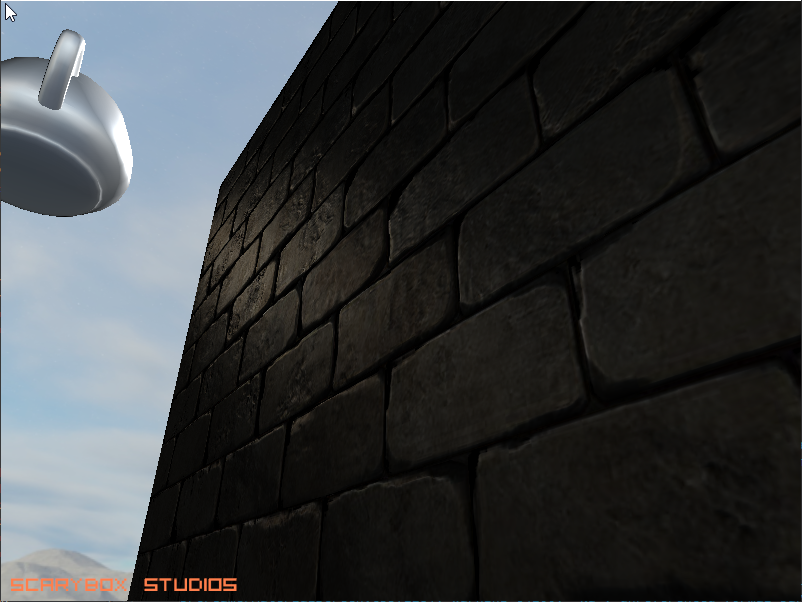
\includegraphics[scale=0.4,clip=true]{./image/nm1.png}
    \caption{Normal Mapping on a metallic wall}
\end{figure}

\begin{figure}[h]
    \centering
    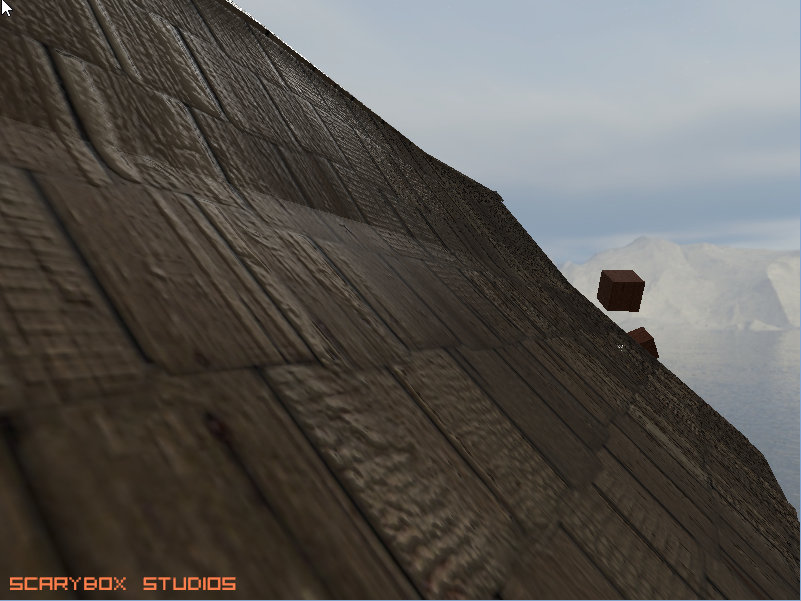
\includegraphics[scale=0.4,clip=true]{./image/nm2.png}
    \caption{Normal Mapping on a house model}
\end{figure}

\newpage
